% !TeX root = main.tex
\section{A Second Example: Another Barcode}

Let us now consider the Hamiltonian diffeomorphism $\phi^2$, where $\phi$ is the diffeomorphism considered in the previous section, i.e.
\begin{equation}
\phi(x,y) = ( x + a \sin(y + a \sin(x)), y + a \sin(x)).
\end{equation}

The Hamiltonian diffeomorphism $\phi$ is the time $2a$ flow of the Hamiltonian $H_1$, defined in $\interval 0 {2a}$. Consequently, $\phi^2$ is the time $4a$ flow of the same Hamiltonian, now extended by periodicity to the interval $\interval 0 {2a}$. Slightly abusing notation, we will write $H_1$ for this extension. A similar observation applies to $H_0$.

We begin by computing the contractible $2a$-periodic orbits of $H_1$ in the torus, i.e. the solutions of $\phi^2(x,y) = (x,y)$ in $\R^2$.

\subsection{The Contractible Periodic Orbits}

\begin{prop}\label{prop:orbitsphi2}
If $a \leq 2$, the solutions to the equation $\phi^2(x,y) = (x,y)$ coincide with the solutions of $\phi(x,y) = (x,y)$, i.e. $(x,y) \in \pi \Z \times \pi \Z$.

If $2 < a < \pi$, there are four new solutions modulo $2\pi$. Let $(x_0, y_0)$ be the unique solution in $\ointerval 0 \pi \times \ointerval 0 \pi$. Then, the other three solutions are given by rotations of this solution about the origin, i.e.
\begin{equation}
(x_0, y_0), (-y_0, x_0), (-x_0, -y_0), \text{ and } (y_0, -x_0).
\end{equation}

Furthermore, $y_0 = \pi - x_0$, and $x_0$ is defined as the unique positive fixed point of $x \mapsto \frac a 2 \sin(x)$.
\end{prop}

\begin{proof}
We begin by writing out the equation $\phi^2(x,y) = (x,y)$ in full:
\begin{equation}\label{phi2id1}
\begin{gathered}
\begin{cases}
x + a \sin(y + a \sin(x)) + a \sin(y_2) = x,\\
y_2 = y,
\end{cases}\\
\text{Where $y_2 = y + a \sin(x) + a \sin(x + a \sin(y + a \sin(x)))$.}
\end{gathered}
\end{equation}

A few elementary computations will show that, for $a > 0$, equation \eqref{phi2id1} is equivalent to
\begin{equation}\label{phi2id2}
\begin{cases}
\sin(y + a \sin(x)) + \sin(y) = 0,\\
\sin(x - a \sin(y)) + \sin(x) = 0.
\end{cases}
\end{equation}

Now, recall that an equation of the form $\sin(A) = - \sin(B)$ has two types of solutions:
\begin{equation}
\begin{aligned}
A &= - B + 2 k \pi, \; k \in \Z && \text{(Type 1)}\\
A &= \pi + B + 2 k \pi, \; k \in \Z && \text{(Type 2).}
\end{aligned}
\end{equation}

Now, the restriction $a < \pi$ implies that neither of the equations in \eqref{phi2id2} has solutions of type 2. For example, a type 2 solution of the first equation would satisfy
\begin{equation}
y + a \sin(x) = \pi + y + 2 k \pi \iff a \sin(x) = \pi + 2 k \pi,
\end{equation}
which is impossible because the left-hand side is always less than $\pi$ in absolute value, while the right-hand side is always greater than or equal to $\pi$ in absolute value.

Therefore, the system \eqref{phi2id2} reduces to
\begin{equation}
\begin{cases}
y = - \frac a 2 \sin(x) + k_1 \pi,\\
x = \frac a 2 \sin(y) + k_2 \pi.
\end{cases}
\end{equation}

Modulo $2\pi$, there are only two cases, $(k_1, k_2) \in \{0,1\} \times \{0,1\}$.

We begin by showing that if $k_1 = k_2$ then there are only the trivial solutions $x = y = k_1 \pi$.

\begin{lemma}
For $k = 0, 1$ and $0 < a < \pi$, the system of equations
\begin{equation}
\begin{cases}
y = - \frac a 2 \sin(x) + k \pi,\\
x = \frac a 2 \sin(y) + k \pi,
\end{cases}
\end{equation}
has only the trivial solution $x = y = k \pi$.
\end{lemma}

\begin{lemmaproof}
It suffices to consider the case $k = 0$, as the other case can be reduced to this one via a change of variables. Suppose then that
\begin{equation}
\begin{cases}
y = - \frac a 2 \sin(x),\\
x = \frac a 2 \sin(y).
\end{cases}
\end{equation}

In this case, $x = - \frac a 2 \sin\left(\frac a 2 \sin(x)\right)$. Such a solution must satisfy $\abs x \leq \frac a 2 < \frac \pi 2$, and therefore the sign of $\sin(x)$ coincides with the sign of $x$. For the same reason $(\abs{\frac a 2 \sin(x)} \leq \frac a 2 < \frac \pi 2)$, the sign of $\sin\left(\frac a 2 \sin(x) \right)$ coincides with the sign of $\frac a2 \sin(x)$, which coincides with the sign of $x$. Unless $x=0$, this is an obvious contradiction.
\end{lemmaproof}

We now handle the case $k_1 \neq k_2$.

\begin{lemma}
For $k = 0, 1$ and $0 < a \leq 2$, the system of equations
\begin{equation}\label{phi2id3}
\begin{cases}
y = - \frac a 2 \sin(x) + k \pi,\\
x = \frac a 2 \sin(y) + (1-k) \pi,
\end{cases}
\end{equation}
has only the trivial solution $x = y = k \pi$.

On the other hand, if $2 < a < \pi$, there exist two new solutions for each value of $k$. The solutions $(x,y)$ to the case $k=0$ are in bijection with the solutions to the case $k=1$, via the map
\begin{equation}
(x,y) \mapsto (y, 2\pi - x).
\end{equation}

Furthermore, if $(x_0, y_0)$ is the unique solution to the $k=0$ case with $x_0 > 0$, we have $y_0 = \pi - x_0$. Finally, the three solutions to the $k_0$ case are $(-x_0, -y_0)$, $(0,0)$ and $(x_0, y_0)$.
\end{lemma}

\begin{lemmaproof}
The bijection between the solutions of the $k=0$ and $k=1$ cases holds regardless of the value of $a$, so both for $0<a\leq 2$ and for $2<a<\pi$ it suffices to verify the case $k=1$.

To find solutions of \eqref{phi2id3} for $k=1$, consider the map
\begin{equation}
\eta(x) = \frac a 2 \sin(x).
\end{equation}

Then, solutions of \eqref{phi2id3} are in one-to-one correspondence with fixed points of $\eta^2 = \eta \circ \eta$, so it suffices to consider that problem instead. Furthermore, since $\eta$ is odd, and consequently so is $\eta^2$, it suffices to look for positive solutions, which must obviously be in the interval $\linterval 0 {\frac a 2}$. Here are some facts about $\eta$ and $\eta^2$, which can be deduced by elementary calculus.
\begin{itemize}
\item The derivatives of $\eta$ and $\eta^2$ at zero are given by $\frac a 2$ and $\left( \frac a 2 \right)^2$ respectively,
\item Both of these functions are concave in $\interval 0 {\frac a 2}$, because their second derivative is negative (strictly except at zero),
\item Both of these functions are increasing in the interval $\interval 0 {\frac a 2}$. This uses the fact that $a < \pi$.	
\end{itemize}

The case $a < 2$ is now easy to solve, as in this event the derivative of $\eta^2(x) - x$ is negative at zero and decreasing in $\interval 0 {\frac a 2}$. Therefore, $\eta^2(x) - x$ is a decreasing function, and since it takes the value $0$ at $x = 0$, it cannot be zero again in the interval.

The case $a = 2$ is similar, though not as direct because the derivative of $\eta^2(x) - x$ at zero is now zero, instead of negative. However, by concavity, this function is still strictly decreasing in $\interval 0 {\frac a 2}$ and the same argument goes through.

Finally, we consider $2 < a < \pi$. In this case, the derivative of $\eta(x) - x$ is positive at zero, and therefore, for small enough values of $x$, $\eta(x) > x$. On the other hand, since $\abs{\eta(x)} \leq \frac a 2$ for all $x$, obviously $\eta(\frac a 2) \leq \frac a 2$. Therefore, by continuity, we have established the existence of a fixed point of $\eta$ in $\linterval 0 {\frac a 2}$, and consequently of a fixed point of $\eta^2$.

We now show that such a fixed point is unique. Since $\eta^2(x)$ is concave in the interval, so is $\eta^2(x) - x$. It is a known fact that a strictly concave function on an interval attains each value at most twice, and so in particular has at most two roots. One of the roots is $x = 0$, and the other is the root which we have proven exists. We call this root $x_0$. To it is associated a solution $(x_0, y_0)$ of \eqref{phi2id3}, satisfying $y_0 = \pi - \eta(x_0)$ and $x_0 = \eta(y_0)$. Note that we have shown that $\eta(x_0) = x_0$, and therefore that $y_0 = \pi - x_0$. This completes the proof of the lemma...
\end{lemmaproof}
...and therefore of the proposition.
\end{proof}

Now that we have computed the contractible periodic orbits of $H_1$, we may label them. We have already labeled the fixed points of $\phi$, and called them $B_0, \dots, B_3$. We have four new periodic orbits, which come in pairs, because they stem from pairs of points $p_1, p_2$ satisfying $\phi(p_1) = p_2$ and $\phi(p_2) = p_1$.

Let $A_0$ refer to the orbit starting at $(x_0, y_0)$, where $(x_0, y_0)$ is as above, and let $A_1$ refer to the orbit starting at $(-x_0, -y_0)$. Likewise, let $C_0$ be the orbit starting at $(-y_0, x_0)$ and $C_1$ be the orbit starting at $(y_0, -x_0)$. For convenience, these labels are represented in figure \ref{orbitsh12}.

\begin{figure}
\centering
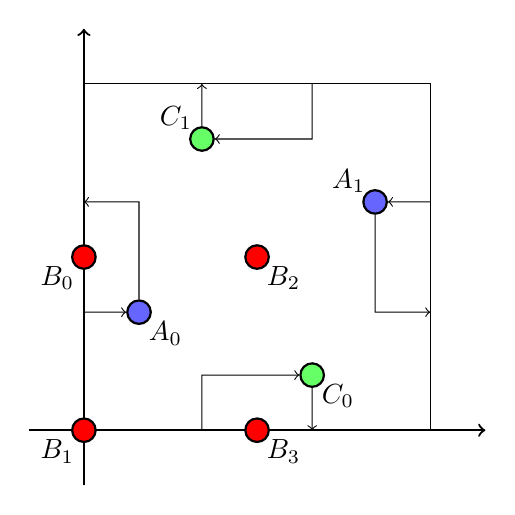
\begin{tikzpicture}[scale=0.7, vertex/.style={draw,circle,thick,fill=red,inner sep=3pt}]
\draw[->,thick] (-1,0) -- (2*pi+1,0);
\draw[->,thick] (0,-1) -- (0,2*pi+1);
\draw (0,0) rectangle (2*pi,2*pi);

\draw (0,0) node[vertex] {} node[below left] {$B_1$};
\draw (0,pi) node[vertex] {} node[below left] {$B_0$};
\draw (pi,0) node[vertex] {} node[below right] {$B_3$};
\draw (pi,pi) node[vertex] {} node[below right] {$B_2$};

\node[vertex,fill=blue!60] (A0) at (1,pi-1) {};
\node[vertex,fill=blue!60] (A1) at (2*pi-1,pi+1) {};
\draw[->] (0,pi-1) -- (A0);
\draw[->] (A0) node[below right] {$A_0$} -- (1,pi+1) -- (0,pi+1);
\draw[->] (2*pi,pi+1) -- (A1);
\draw[->] (A1) node[above left] {$A_1$} -- (2*pi-1,pi-1) -- (2*pi,pi-1);

\node[vertex,fill=green!60] (C0) at (pi+1,1) {};
\node[vertex,fill=green!60] (C1) at (pi-1,2*pi-1) {};
\draw[->] (C0) -- (pi+1,0);
\draw[->] (pi-1,0) -- (pi-1,1) -- (C0) node[below right] {$C_0$};
\draw[->] (C1) -- (pi-1,2*pi);
\draw[->] (pi+1,2*pi) -- (pi+1,2*pi-1) -- (C1) node[above left] {$C_1$};
\end{tikzpicture}
\caption{The contractible $4a$-periodic orbits of $H_1$, labeled. The label of an orbit is next to its starting point. For the non-constant orbits, the arrow represents the time $2a$-flow.}
\label{orbitsh12}
\end{figure}

\subsection{Their Actions}

We now compute the actions of the orbits $A_0$, $A_1$, $B_0, \dots, B_3, C_0$ and $C_1$.

We begin with the constant orbits $B_i$. By a similar argument as the one done for the case of the Hamiltonian diffeomorphism $\phi$, the action of these orbits is simply the integral of $H_1$, which is given by $2a(\cos(y) - \cos(x)$.

Let us now inspect the orbits $A_i$ and $C_i$. Note that the paths these orbits take are squares, and therefore we may consider the embedded disk $D$ in the definition of the action functional to be a diffeomorphism between the interior of the disk and these squares. Furthermore, since the symplectic form $\omega$ is the area form on the torus, it pulls back to the area form on the square. Consequently, the $- \int_D \omega$ term in the action functional will be equal to the area of the square or its symmetric, depending on the orientation of the border: In the counterclockwise case ($A_0$, $A_1$) the orientation is positive, while in the clockwise case ($C_0$, $C_1$) it is negative. Finally, the area of these squares, in absolute value, is equal to their side squared, i.e. $(2x_0)^2 = 4x_0^2$.

Now we inspect the $\int H_1$ term in the action functional applied to these orbits. For the sake of concreteness, we will compute it for $A_0$, but the same argument goes for the other three.

The orbit $A_0$ can be divided into four (reparametrized) linear segments. For example, the first segment goes from $(x_0, y_0)$ to $(x_0, y_0 + 2a \sin(x_0)) = (x_0, \pi + x_0)$. Over this segment, the Hamiltonian $H_1$ takes the value $- \varphi(t) \cos(x_0)$ at time $t$, (see equation \eqref{h1def}) and integrating we obtain a contribution of $- a \cos(x_0)$ to $\int H_1$. It is easy to compute the contributions of the four other line segments. They are all also equal to $- a \cos(x_0)$, and so we conclude
\begin{equation}
\AA(A_0) = - 4 x_0^2 - 4 a \cos(x_0).
\end{equation}

It is easy to check that this value coincides with $\AA(A_1)$, and furthermore that
\begin{equation}
\AA(C_0) = \AA(C_1) = - \AA(A_0).
\end{equation}

As a last remark, we prove a simple inequality regarding $\AA(A_0)$, so that we can place the actions we have calculated so far on a line.

\begin{prop}
Let $2 < a < \pi$ and $x_0$ be as in proposition \ref{prop:orbitsphi2}. Then, we have the inequality
\begin{equation}
0 < 4 x_0^2 + 4 a \cos(x_0) < 4a.
\end{equation}
\end{prop}

\begin{proof}
Since $0 < x_0 < \pi$, it should be obvious that $4 x_0^2 + 4 a \cos(x_0) > 0$, as it is a sum of two positive terms. Therefore, we turn to proving the other inequality.

Recall that $x_0$ satisfies the equality $x_0 = \frac a 2 \sin(x_0)$. Consequently, $4 x_0^2 = a^2 \sin^2 (x_0) = a^2 - a^2 \cos^2(x_0)$. Therefore,
\begin{equation}
4 x_0^2 + 4 a \cos(x_0) = a^2 + 4 a \cos(x_0) - a^2 \cos^2(x_0).
\end{equation}

Therefore, to show that $4 x_0^2 + a \cos(x_0) < 4a$ it suffices to show
\begin{equation}
\begin{aligned}
&& a^2 + 4 a \cos(x_0) - a^2 \cos^2(x_0) &< 4a\\
\iff&& 4 (\cos(x_0)-1) + a(1 - \cos^2(x_0)) &< 0\\
\iff&& (\cos(x_0) - 1)(4 - a(1 + \cos(x_0))) &< 0\\
\iff&& 4 - a(1+ \cos(x_0)) &> 0\\
\iff&& a + a \cos(x_0) &< 4.
\end{aligned}
\end{equation}

The proof of this last inequality is somewhat involved. We begin by writing $a$ as a function of $x_0$, as
\begin{equation}
a = \frac{2 x_0}{\sin(x_0)}.
\end{equation}

Therefore, we intend to show that, for $x_0$ in, say, $\interval 0 {\frac \pi 2}$, the expression $\frac{x_0}{\sin(x_0)}(1 + \cos(x_0))$ is always less than 2. To this effect, we study the function
\begin{equation}
f(t) = \frac{t}{\sin(t)}(1 + \cos(t)).
\end{equation}

Laborious but straightforward computations will show that the derivative of $f$ is given by
\begin{equation}
f'(t) = - \frac{t - \sin(t)}{1 - \cos(t)}.
\end{equation}

Evidently, for $t > 0$, $f'(t) < 0$ where defined. Consequently, $f$ is a strictly decreasing function. Since $\lim_{t \to 0^+} f(t) = 2$, we obtain that $f(t) < 2$ for $t \in \ointerval 0 {\frac \pi 2}$, which completes the proof.
\end{proof}

We can now place the actions of the orbits on the real line.

[[place figure here]]